\documentclass{article}

%Packages

\usepackage[utf8]{inputenc}

\usepackage[parfill]{parskip}

\usepackage[colorlinks=true,urlcolor=codeblue]{hyperref}

\usepackage{minted, graphicx}

%Document

\title{`Software Sustainability: If a tree falls in a forest...' -
King's workshop exercise}

\author{Martin Chapman}

\date{Wednesday 9th December 2020}

\begin{document}

\definecolor{bg}{rgb}{0.95,0.95,0.95}
\definecolor{codeblue}{rgb}{0,0.3,0.6}

\maketitle

\section{Prerequisites}

The below material assumes
that the software sustainability course has been completed
(\href{https://www.youtube.com/playlist?list=PLxyHJ\_wep1\_DPbvtFl\_-EGyoz2pVt-n1\_}{https://www.youtube.com/playlist?list=PLxyHJ\_wep1\_DPbvtFl\_-EGyoz2pVt-n1\_}),
and that Python 3, nodejs, Git, Docker and Docker Compose are all
installed.

\section{Background}

\begin{center}
    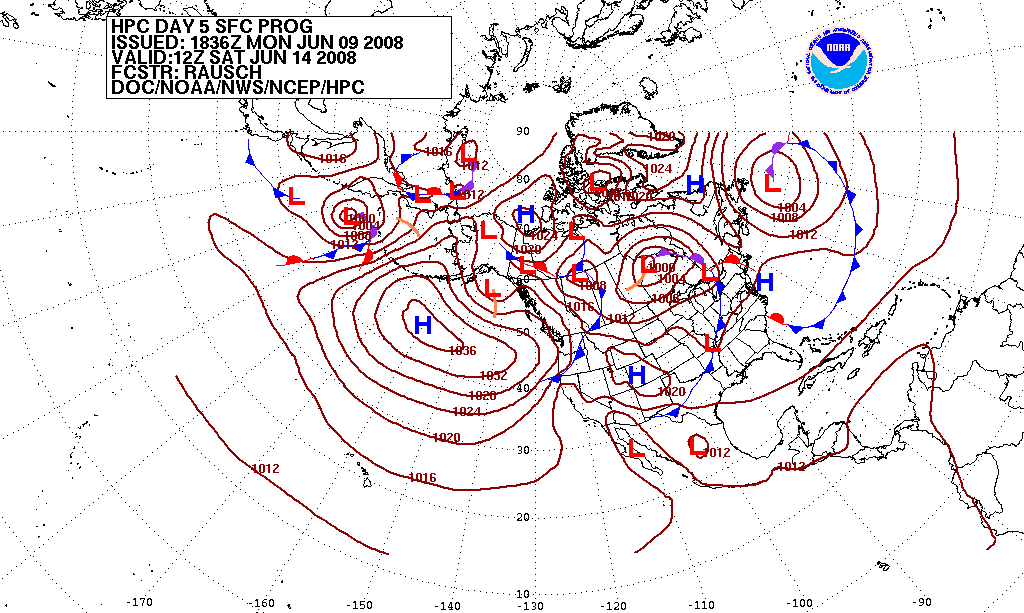
\includegraphics[height=5cm]{weather.png}
\end{center}

We are going to imagine we have just invented a perfect model of the
weather, that allows us to make predictions for a specific location on
a specific day.

Our model takes as input a location (e.g. ``London'') and the number of
days from now at which to make a prediction about the weather in that
location (e.g. 3 (days from now)).

To make a prediction, the model first takes the
\href{https://en.wikipedia.org/wiki/List_of_Unicode_characters}{Unicode}
value of the first letter of the location (e.g. `L', which is 76 in
Unicode) and computers the remainder of this value when divided by
3. This produces a number between 0 and 2. Next, the model takes the
number of days from now at which to make a prediction, and also computes
the remainder of this value when divided by 3.  This also produces a
number between 0 and 2. These two numbers are then added together to
produce a number between 0 and 4.

To make a final prediction, each number produced by the model is matched
to a specific type of weather:

0 = sun, 1 = wind, 2 = rain, 3 = snow and 4 = cloud.

\subsection{Example}

\begin{enumerate}

    \item A user enters \mintinline[bgcolor=bg]{bash}{London} and
    \mintinline[bgcolor=bg]{bash}{3}.

    \item The value of `L' in Unicode is 76. The remainder of 76 / 3 is 1.

    \item The remainder of 3 / 3 is 0.

    \item Our final prediction value is 1 (1 + 0), which corresponds to
    `wind'.

\end{enumerate}

\section{Session 1 (10.10 - 10.30) - Coding practice}

Realise the weather model described in Python code, adhering to the
principles of coding practice discussed in the course.

Hint: the \mintinline[bgcolor=bg]{python}{ord()} function is useful for
converting a character to its Unicode value.

Your code should accept a location and a number of days as user input,
and use the model to make a prediction based on this input.

\section{Session 2 (11.00 - 11.25) - Version control}

Make a version of your software, and push it to a remote repository
on King's Github (\href{https://github.kcl.ac.uk/}{github.kcl.ac.uk}).
Call this repository `\textbf{simulation}'.

You will need to log in with your k-number and password, if you have
not done so before.

\textit{Public Github (\href{https://github.com}{github.com}), should
also work for this task, but should only be used as a backup.}

Additional versions should be made at appropriate points while completing
the remaining tasks.

\subsection{Assessment}

To receive a mark for your work, add the user \textbf{MC} as a
collaborator to your repository.

To add someone as a collaborator, from your repository visit
\textit{Settings} $>$ \textit{Collaborators \& Teams}. You may need to
log in again. In the \textit{Collaborators} box, under \textit{Search
by username, full name or email address}, search for the user
`\textbf{MC}'. Click the first result in the dropdown box and then
click \textit{Add collaborator}. Verify that `MC' is a collaborator on
your repository.

\textit{If using public Github as a backup, the path to add a collaborator
will instead be \textit{Settings} $>$ \textit{Manage access}. Click
\textit{Invite a collaborator}, and in the box that pops up search for
the user `\textbf{martinchapman}' and click the top result. Verify that
`martinchapman' is a collaborator on your repository.}

If you are asked to set an access level for the collaborator, choose
\textit{Admin}.

Via this collaborator link, your repository will be accessed and your
mark will be based on the number of passing tests in your code.

\section{Session 3 (12.00 - 12.25) - Testing}

Write three tests to ensure the following:

\begin{enumerate}

    \item The weather in London in 5 days time is ``snow''.

    \item The weather in London in 365 days time is ``snow''.

    \item The weather in London in -1 days time is not reported.

\end{enumerate}

Modify your program such that these tests pass, if needed.

You are welcome to add additional tests, but these must all pass.

\section{Session 4 (14.00 - 14.25) - Services}

The supporting material for this session is available at
\href{https://github.com/martinteaching/sustainability2020}{github.com/martinteaching/sustainability2020}.

Wrap your Python weather prediction model in a server and run it.

Move the request for user input (location and days) to a Javascript
client, which, once acquired, sends this information to the server,
waits for it to compute the result using the model, and then prints the
result for the user.

\section{Session 5 (15.00 - 15.25) - Docker}

Dockerise your program, using a Dockerfile and Docker compose, allowing
the Python server to run in a container, and the Javascript client to
issue requests to it.

\section{Additional Tasks}

If you wish to expand on your solution, separate your Python weather model
server code into two servers (services). Each service should contain
code to compute part of the weather prediction (e.g. one service for
the location calculation, another for the day calculation). Designate
one of your services as the `user-facing' service, to be called by
the client (Service A). Service A, when called by a client, should
then subsequently call the other service (Service B) for its result,
before combining Service B's result with its own, and returning this in
a response to the client.

For example, Service A could compute the location value, call Service
B to compute the day value, combine the results, and return them to a
requesting client.

\end{document}
